%%%%%%%%%%%%%%%%%%%%%%%%%%%%%%%%%%%%%%%%%%%%%%%%%%%%%%%%%%%%%%%%%%%%%%%%%%%%%%%%%%
\begin{frame}[fragile]\frametitle{}
\begin{center}
{\Large Introduction}
\end{center}
\end{frame}

%%%%%%%%%%%%%%%%%%%%%%%%%%%%%%%%%%%%%%%%%%%%%%%%%%%%%%%%%%%%%%%%%%%%%%%%%%%%%%%%%%
\begin{frame}[fragile]\frametitle{Overview of Time Series Analysis}
    \begin{itemize}
        \item Time series data: Sequential observations over time
        \item Challenges in time series analysis:
            \begin{itemize}
                \item Pattern discovery
                \item Anomaly detection
                \item Similarity search
            \end{itemize}
        \item Need for efficient algorithms and tools
    \end{itemize}
\end{frame}

%%%%%%%%%%%%%%%%%%%%%%%%%%%%%%%%%%%%%%%%%%%%%%%%%%%%%%%%%%%%%%%%%%%%%%%%%%%%%%%%%%
\begin{frame}[fragile]\frametitle{Introduction to Time Series Data Mining}
    \begin{itemize}
        \item Time series data is ubiquitous across domains like:
            \begin{itemize}
                \item \textbf{Medical:} Gene expression, ECG, EEG, gait analysis, growth charts.
                \item \textbf{Other fields:} Industry, finance, meteorology, entertainment, etc.
            \end{itemize}
        \item Explosion of interest due to growing databases and their sizes.
        \item Traditional statistical techniques have limited utility for massive datasets.
    \end{itemize}
\end{frame}

%%%%%%%%%%%%%%%%%%%%%%%%%%%%%%%%%%%%%%%%%%%%%%%%%%%%%%%%%%%%%%%%%%%%%%%%%%%%%%%%%%
\begin{frame}[fragile]\frametitle{What do you do \ldots}
If you see the following \ldots
      \begin{center}
        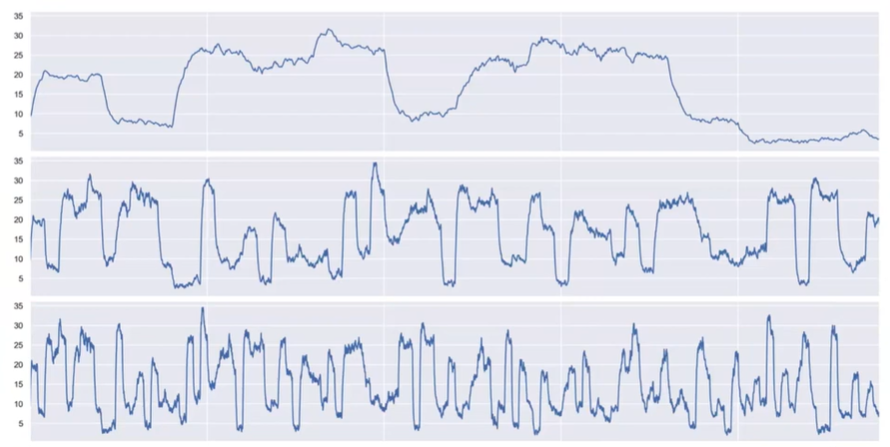
\includegraphics[width=0.8\linewidth,keepaspectratio]{timeseries_resolution}

		{\tiny (Ref: Thomas J. Fan - Time Series EDA with STUMPY)}		
        \end{center}
	
They are the same time series at different resolutions. Hard to process, right? But they are everywhere? How to process them? What can we do with them?	
\end{frame}


%%%%%%%%%%%%%%%%%%%%%%%%%%%%%%%%%%%%%%%%%%%%%%%%%%%%%%%%%%%%%%%%%%%%%%%%%%%%%%%%%%
\begin{frame}[fragile]\frametitle{Major Tasks in Time Series Data Mining}
    \begin{itemize}
        \item \textbf{Indexing (Query by Content):}
            \begin{itemize}
                \item Find the most similar time series in a database using a similarity measure.
            \end{itemize}
        \item \textbf{Clustering:}
            \begin{itemize}
                \item Group time series into natural clusters based on similarity.
            \end{itemize}
        \item \textbf{Classification:}
            \begin{itemize}
                \item Assign unlabeled time series to predefined classes.
            \end{itemize}
    \end{itemize}
\end{frame}

%%%%%%%%%%%%%%%%%%%%%%%%%%%%%%%%%%%%%%%%%%%%%%%%%%%%%%%%%%%%%%%%%%%%%%%%%%%%%%%%%%
\begin{frame}[fragile]\frametitle{Advanced Tasks in Time Series Data Mining}
    \begin{itemize}
        \item \textbf{Prediction (Forecasting):}
            \begin{itemize}
                \item Predict the next data point based on existing time series.
            \end{itemize}
        \item \textbf{Summarization:}
            \begin{itemize}
                \item Create a simplified visual representation of a large time series.
            \end{itemize}
        \item \textbf{Anomaly Detection:}
            \begin{itemize}
                \item Identify anomalies or unexpected occurrences in a time series.
            \end{itemize}
    \end{itemize}
\end{frame}

%%%%%%%%%%%%%%%%%%%%%%%%%%%%%%%%%%%%%%%%%%%%%%%%%%%%%%%%%%%%%%%%%%%%%%%%%%%%%%%%%%
\begin{frame}[fragile]\frametitle{Segmentation in Time Series Analysis}
    \begin{itemize}
        \item Two approaches:
            \begin{itemize}
                \item \textbf{Piecewise Approximation:}
                    \begin{itemize}
                        \item Approximate a time series using \( K \) segments (\( K << n \)).
                    \end{itemize}
                \item \textbf{Partitioning:}
                    \begin{itemize}
                        \item Divide time series into \( K \) homogeneous sections.
                    \end{itemize}
            \end{itemize}
        \item Often used for change detection.
    \end{itemize}
\end{frame}

%%%%%%%%%%%%%%%%%%%%%%%%%%%%%%%%%%%%%%%%%%%%%%%%%%%%%%%%%%%%%%%%%%%%%%%%%%%%%%%%%%
\begin{frame}[fragile]\frametitle{Importance of Distance Measures}
    \begin{itemize}
        \item \textbf{Indexing and Clustering:}
            \begin{itemize}
                \item Explicitly rely on similarity/dissimilarity measures.
            \end{itemize}
        \item \textbf{Other Tasks:}
            \begin{itemize}
                \item Implicitly use similarity measures (classification, prediction, etc.).
            \end{itemize}
        \item Fundamental to most time series data mining methods.
    \end{itemize}
\end{frame}
%%%%%%%%%%%%%%%%%%%%%%%%%%%%%%%%%%%%%%%%%%%%%%%%%%%%%%%%%%%%%%%%%%%%%%%%%%%%%%%%%%
\begin{frame}[fragile]\frametitle{Introduction to the Matrix Profile}
    \begin{itemize}
        \item \textbf{Matrix Profile:} A time-series data structure that annotates each subsequence of a time series.
        \item Records:
            \begin{itemize}
                \item \textbf{Location} of the nearest neighbor.
                \item \textbf{Distance} to the nearest neighbor.
            \end{itemize}
        \item Enables efficient resolution of:
            \begin{itemize}
                \item Time series \textbf{motif queries}.
                \item Time series \textbf{discord queries}.
            \end{itemize}
    \end{itemize}
\end{frame}


%%%%%%%%%%%%%%%%%%%%%%%%%%%%%%%%%%%%%%%%%%%%%%%%%%%%%%%%%%%%%%%%%%%%%%%%%%%%%%%%%%
\begin{frame}[fragile]\frametitle{What is Matrix Profile?}
    \begin{itemize}
        \item A powerful technique for time series analysis
        \item Developed to solve multiple time series challenges
        \item Key features:
            \begin{itemize}
                \item Exact similarity search
                \item Motif discovery
                \item Discord detection
            \end{itemize}
    \end{itemize}
\end{frame}

%%%%%%%%%%%%%%%%%%%%%%%%%%%%%%%%%%%%%%%%%%%%%%%%%%%%%%%%%%%%%%%%%%%%%%%%%%%%%%%%%%
\begin{frame}[fragile]\frametitle{Advantages of the Matrix Profile}
    \begin{itemize}
        \item Encodes all information for motif and discord discovery.
        \item Efficiently handles long subsequences without suffering from the \textbf{curse of dimensionality}.
        \item Supports analysis across diverse domains:
            \begin{itemize}
                \item \textbf{Bioinformatics:} Discovery of motifs as long as 60,000 datapoints.
                \item \textbf{Large-scale datasets:} Processing datasets 100x larger than previous limits.
            \end{itemize}
    \end{itemize}
\end{frame}

%%%%%%%%%%%%%%%%%%%%%%%%%%%%%%%%%%%%%%%%%%%%%%%%%%%%%%%%%%%%%%%%%%%%%%%%%%%%%%%%%%
\begin{frame}[fragile]\frametitle{Generality and Utility of the Matrix Profile}
    \begin{itemize}
        \item \textbf{Extraordinary generality:} Enables numerous analytical tasks with minimal additional code.
        \item Example: Most tasks can be implemented with:
            \begin{itemize}
                \item \textbf{Matrix Profile:} Precomputed.
                \item \textbf{10 lines of additional code:} High-level language (e.g., MATLAB).
            \end{itemize}
        \item Simplifies complex algorithms and tasks for analysts.
    \end{itemize}
\end{frame}

%%%%%%%%%%%%%%%%%%%%%%%%%%%%%%%%%%%%%%%%%%%%%%%%%%%%%%%%%%%%%%%%%%%%%%%%%%%%%%%%%%
\begin{frame}[fragile]\frametitle{Philosophical Impact of the Matrix Profile}
    \begin{itemize}
        \item \textbf{Comparison to sorting algorithms:}
            \begin{itemize}
                \item Programmers treat sorting as a \textbf{computationally "free"} operation.
                \item Matrix Profile aims to provide a similar abstraction for time-series tasks.
            \end{itemize}
        \item Encourages experimentation:
            \begin{itemize}
                \item \textbf{Quick results:} Faster computation and coding time.
                \item \textbf{Reduces barriers:} Analysts can test ideas without significant delays.
            \end{itemize}
        \item Potentially \textbf{game-changing} for time-series data mining.
    \end{itemize}
\end{frame}

%%%%%%%%%%%%%%%%%%%%%%%%%%%%%%%%%%%%%%%%%%%%%%%%%%%%%%%%%%%%%%%%%%%%%%%%%%%%%%%%%%
\begin{frame}[fragile]\frametitle{Computation of the Matrix Profile}
    \begin{itemize}
        \item Multiple algorithms can compute the Matrix Profile:
            \begin{itemize}
                \item \textbf{STAMP} 
                \item \textbf{STOMP} 
                \item \textbf{STOMPI} 
                \item \textbf{SCRIMP++} 
            \end{itemize}
        \item Analysts can use these methods interchangeably:
            \begin{itemize}
                \item Abstracts computational details.
                \item Focus remains on solving higher-level problems.
            \end{itemize}
		\item One of the most performant implementation is by \textbf{STUMPY}, lets see that next!!
    \end{itemize}
\end{frame}

%%%%%%%%%%%%%%%%%%%%%%%%%%%%%%%%%%%%%%%%%%%%%%%%%%%%%%%%%%%%%%%%%%%%%%%%%%%%%%%%%%
\begin{frame}[fragile]\frametitle{Introduction to Stumpy}
    \begin{itemize}
        \item Python library for Matrix Profile computation
        \item Key characteristics:
            \begin{itemize}
                \item Efficient implementation
                \item NumPy-compatible interface
                \item Scalable for large datasets
            \end{itemize}
        \item Open-source implementation
    \end{itemize}
\end{frame}

%%%%%%%%%%%%%%%%%%%%%%%%%%%%%%%%%%%%%%%%%%%%%%%%%%%%%%%%%%%%%%%%%%%%%%%%%%%%%%%%%%
\begin{frame}[fragile]\frametitle{Applications}
    \begin{itemize}
        \item Pattern recognition in sensor data
        \item Financial time series analysis
        \item Bioinformatics sequence analysis
        \item Industrial monitoring
        \item Geophysical data processing
    \end{itemize}
\end{frame}

%%%%%%%%%%%%%%%%%%%%%%%%%%%%%%%%%%%%%%%%%%%%%%%%%%%%%%%%%%%%%%%%%%%%%%%%%%%%%%%%%%
\begin{frame}[fragile]\frametitle{Why Matrix Profile?}
    \begin{itemize}
        \item Advantages:
            \begin{itemize}
                \item Parameter-light algorithm
                \item Handles variable-length patterns
                \item Scale-invariant similarity search
            \end{itemize}
        \item Efficient computation with Stumpy
        \item Interpretable results
    \end{itemize}
\end{frame}
